\chapter{Генерация случайных чисел по заданному ряду распределения}
\label{ch:chap2}

Реализация:\\

\begin{figure}[H]
    \centering
    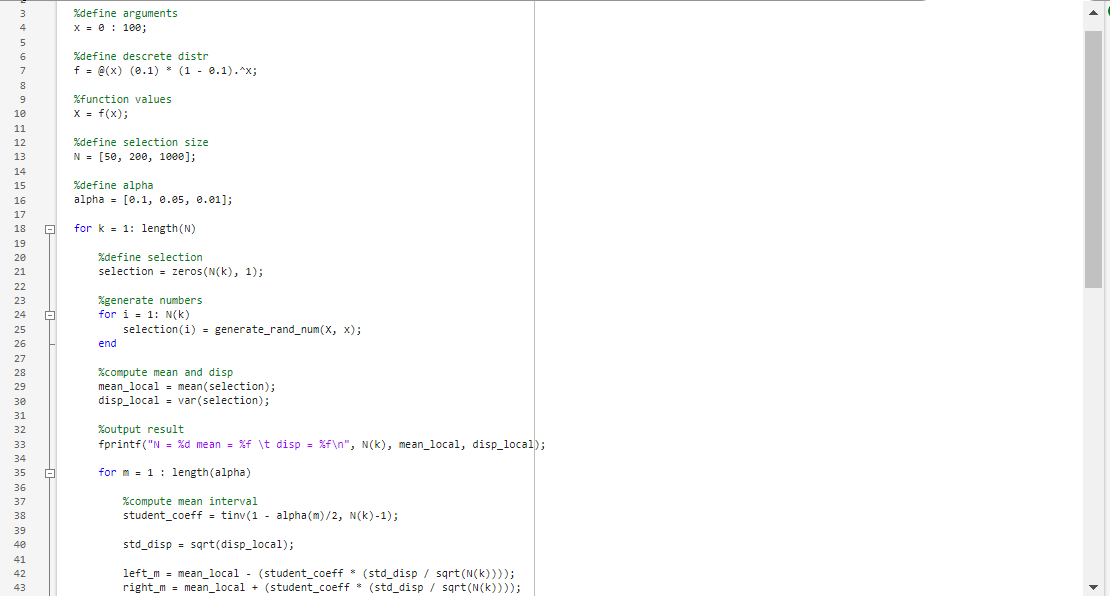
\includegraphics[width=1.0\textwidth]{descr_real_1.png}
    \caption{Реализация программы для ряда распределения (часть 1)}
\end{figure}


\begin{figure}[H]
    \centering
    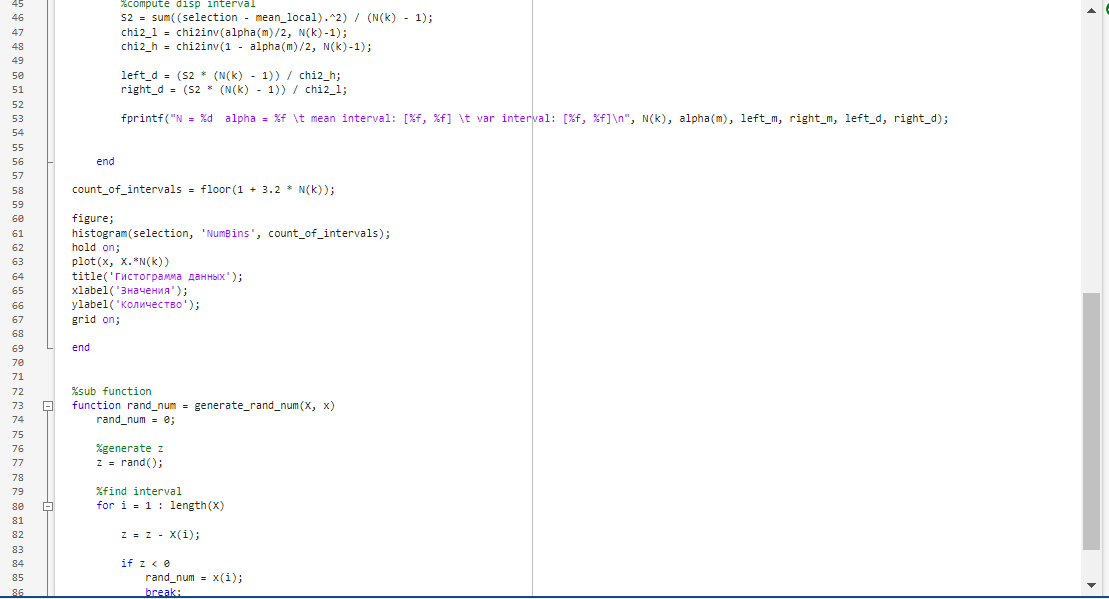
\includegraphics[width=1.0\textwidth]{descr_real_2.png}
    \caption{Реализация программы для ряда распределения (часть 2)}
\end{figure}

Результат: \\

\begin{figure}[H]
    \centering
    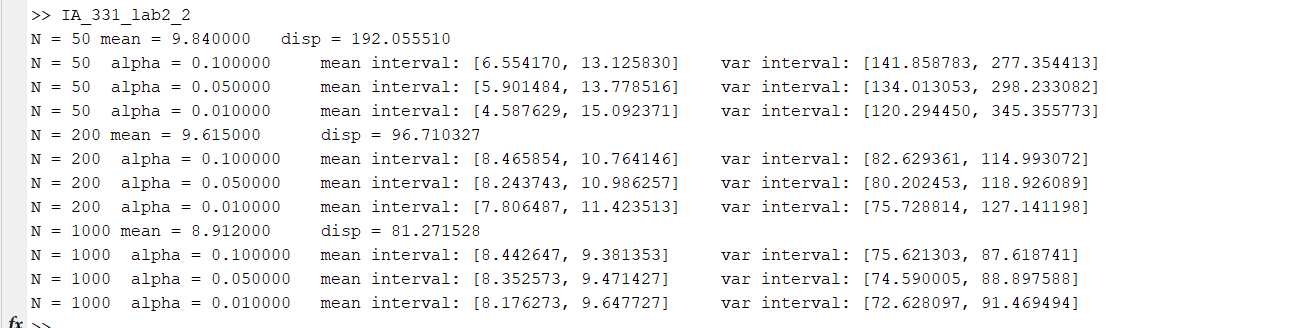
\includegraphics[width=1.0\textwidth]{cmd_res_descr.png}
    \caption{Базовые параметры случайной величины для выборок разного объема (N = 50, 200, 1000)}
\end{figure}


\begin{figure}[H]
    \centering
    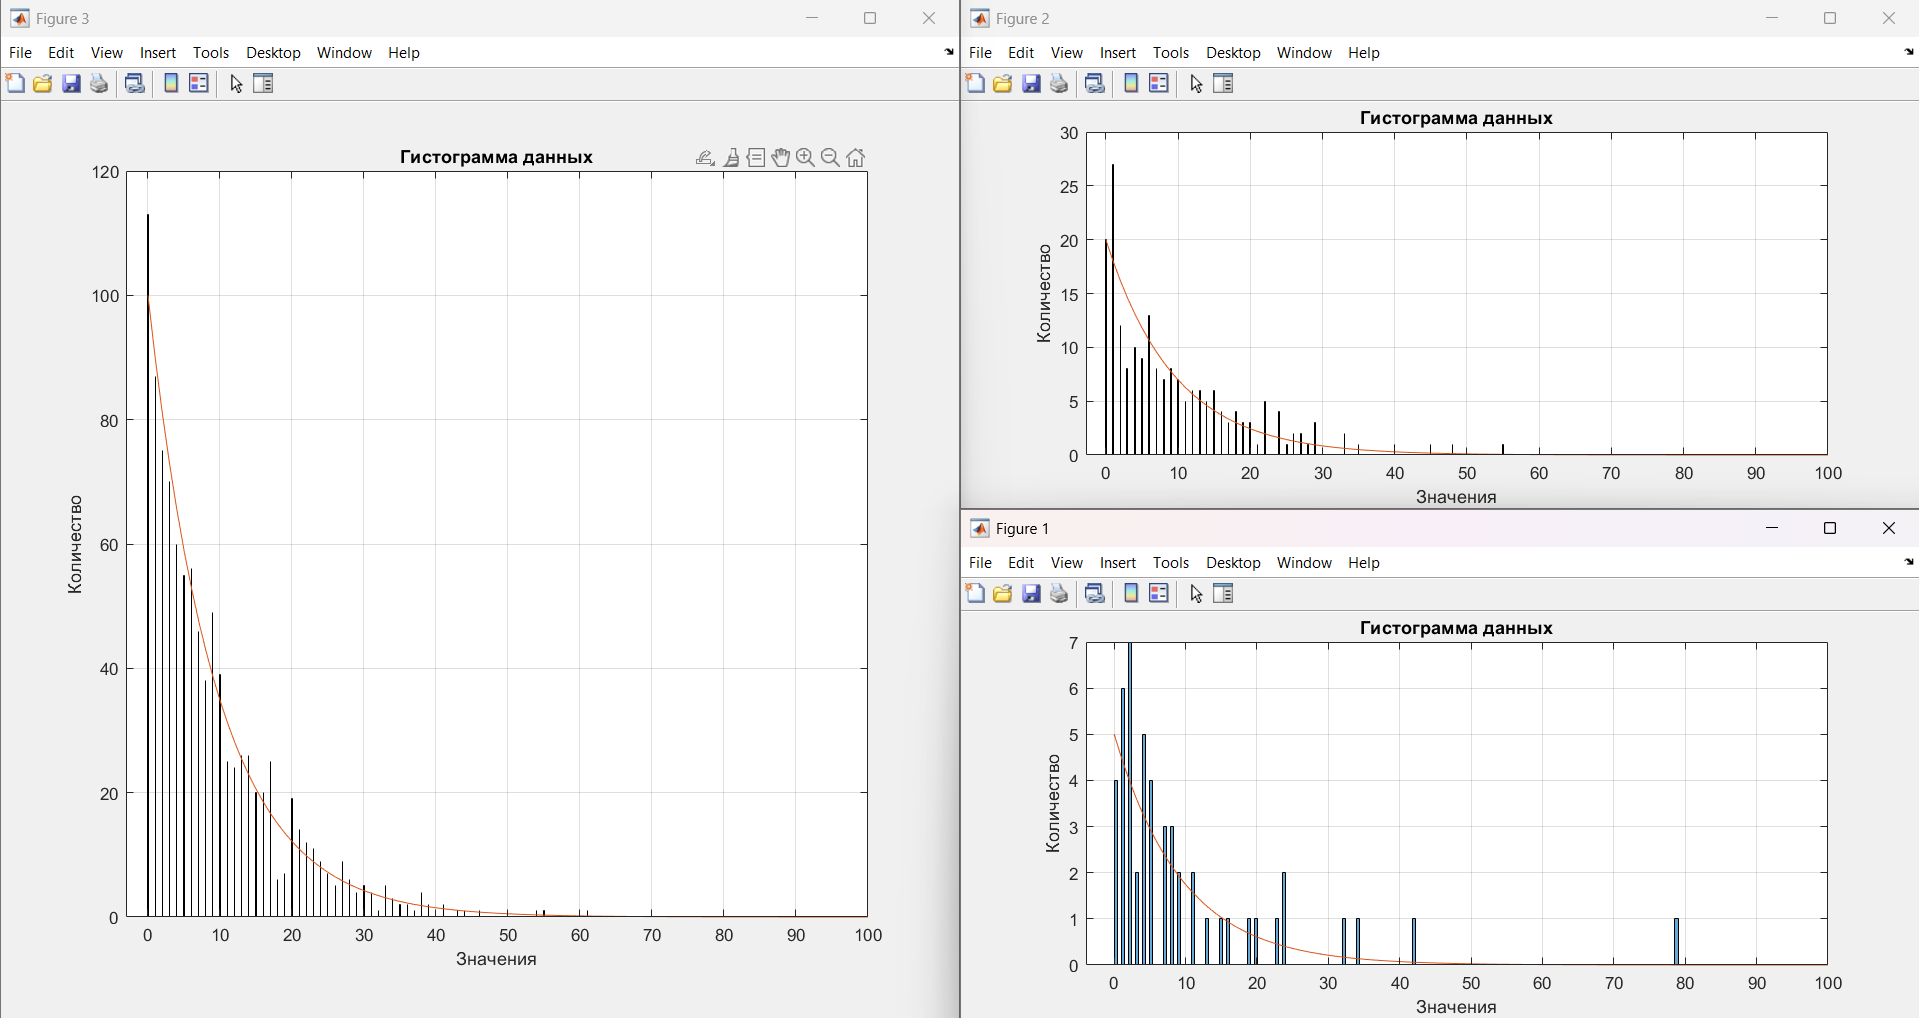
\includegraphics[width=1.0\textwidth]{descr_graph.png}
    \caption{Гистограммы и закон распределения для выборок разного объема}
\end{figure}

\endinput